\documentclass[tikz,border=6pt]{standalone}
% shared TikZ style for the diagrams (colours match the plots)
\usepackage[T1]{fontenc}
\usepackage{lmodern}
\usepackage{amsmath,amssymb}
\usepackage{tikz}
\usetikzlibrary{arrows.meta,positioning,fit,backgrounds,calc,shapes.misc,decorations.pathreplacing}
\definecolor{cBlue}{HTML}{2A78D6}
\definecolor{cOrange}{HTML}{EB6834}
\definecolor{cAqua}{HTML}{1BAF7A}
\definecolor{cViolet}{HTML}{6250D6}
\definecolor{cGreen}{HTML}{008300}
\definecolor{cGray}{HTML}{8F8D86}
\definecolor{cInk}{HTML}{0B0B0B}
\definecolor{cInk2}{HTML}{52514E}
\tikzset{
  box/.style={draw=#1!70!black, fill=#1!10, rounded corners=3pt, align=center, inner sep=4pt, font=\small, line width=0.6pt},
  box/.default=cGray,
  arr/.style={-{Stealth[length=2.4mm]}, line width=0.8pt, cInk2},
  lbl/.style={font=\scriptsize, text=cInk2, align=center},
}

\begin{document}
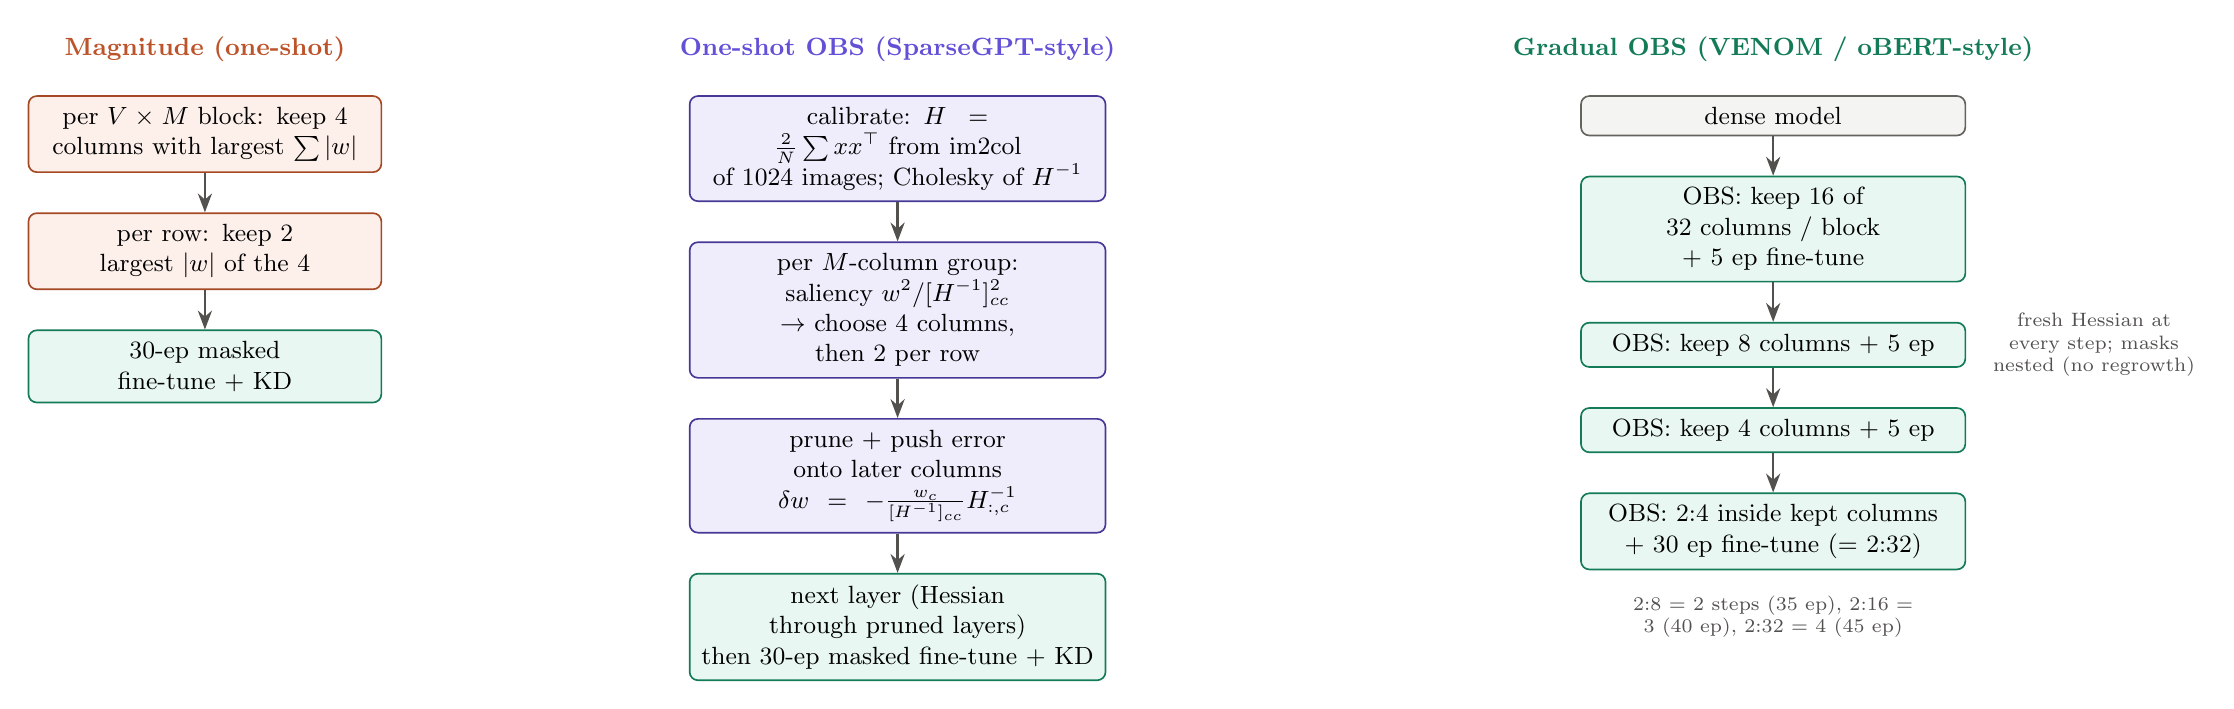
\begin{tikzpicture}[node distance=5mm and 6mm]
% magnitude
\node[font=\small\bfseries, text=cOrange!80!black] (t1) {Magnitude (one-shot)};
\node[box=cOrange, text width=42mm, below=3mm of t1] (m1) {per $V\times M$ block: keep 4 columns with largest $\sum|w|$};
\node[box=cOrange, text width=42mm, below=of m1] (m2) {per row: keep 2 largest $|w|$ of the 4};
\node[box=cAqua, text width=42mm, below=of m2] (m3) {30-ep masked fine-tune + KD};
\draw[arr] (m1)--(m2); \draw[arr] (m2)--(m3);
% one-shot OBS
\node[font=\small\bfseries, text=cViolet, right=40mm of t1] (t2) {One-shot OBS (SparseGPT-style)};
\node[box=cViolet, text width=50mm, below=3mm of t2] (o1) {calibrate: $H=\tfrac{2}{N}\sum xx^\top$ from im2col\\of 1024 images; Cholesky of $H^{-1}$};
\node[box=cViolet, text width=50mm, below=of o1] (o2) {per $M$-column group: saliency $w^2/[H^{-1}]_{cc}^2$\\$\to$ choose 4 columns, then 2 per row};
\node[box=cViolet, text width=50mm, below=of o2] (o3) {prune + push error onto later columns\\$\delta w=-\tfrac{w_c}{[H^{-1}]_{cc}}H^{-1}_{:,c}$};
\node[box=cAqua, text width=50mm, below=of o3] (o4) {next layer (Hessian through pruned layers)\\then 30-ep masked fine-tune + KD};
\draw[arr] (o1)--(o2); \draw[arr] (o2)--(o3); \draw[arr] (o3)--(o4);
% gradual
\node[font=\small\bfseries, text=cAqua!70!black, right=48mm of t2] (t3) {Gradual OBS (VENOM / oBERT-style)};
\node[box=cGray, text width=46mm, below=3mm of t3] (g0) {dense model};
\node[box=cAqua, text width=46mm, below=of g0] (g1) {OBS: keep 16 of 32 columns / block\\+ 5 ep fine-tune};
\node[box=cAqua, text width=46mm, below=of g1] (g2) {OBS: keep 8 columns + 5 ep};
\node[box=cAqua, text width=46mm, below=of g2] (g3) {OBS: keep 4 columns + 5 ep};
\node[box=cAqua, text width=46mm, below=of g3] (g4) {OBS: 2:4 inside kept columns\\+ 30 ep fine-tune (= 2:32)};
\draw[arr] (g0)--(g1); \draw[arr] (g1)--(g2); \draw[arr] (g2)--(g3); \draw[arr] (g3)--(g4);
\node[lbl, right=2mm of g2, text width=26mm] {fresh Hessian at\\every step; masks\\nested (no regrowth)};
\node[lbl, below=2mm of g4, text width=60mm] {2:8 = 2 steps (35 ep), 2:16 = 3 (40 ep), 2:32 = 4 (45 ep)};
\end{tikzpicture}
\end{document}
